%% ---------------------------------------------------------------------------------------------------------
\section{Calibration certificate and Final Test}\label{sec:confirm}

\paragraph{Question} On new scenes and with nothing changed after development, can a conditional harm rate of 5\% or more be rejected (calibration), and does V2 increase success (Final Test)? The two questions are answered on disjoint scene sets with pre-registered tests; everything else in this section is labelled descriptive or post hoc.

\begin{figure}[!htbp]
\centering
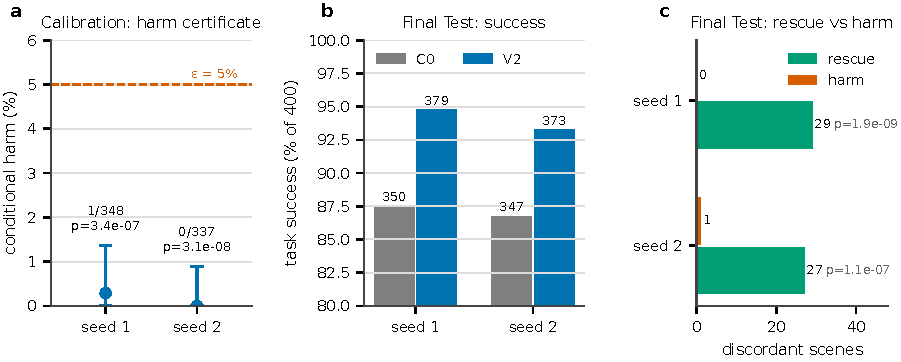
\includegraphics[width=\linewidth]{Fig04_statistics_calibration_vs_test.pdf}
\caption{Confirmatory stages, per policy. (a) Calibration (400 scenes per policy; harm counted among the $n_+$ baseline successes): observed conditional harm, its one-sided 95\% Clopper--Pearson upper bound (post hoc, descriptive) and the pre-registered level $\varepsilon=5\%$; p-values from Eq.~\eqref{eq:cert}, one-sided. (b) Final Test (400 held-out scenes per policy, run once): successes of C0 and V2. (c) Final Test discordant scenes and the one-sided p-values of Eq.~\eqref{eq:eff}.}\label{fig:stats}
\end{figure}

\begin{table}[!htbp]
\centering\footnotesize
\caption{Calibration certificate and Final Test. Trig.: scenes with a trigger; Acted: scenes in which V2 moved; C0, V2: successes of 400. Calibration tests $H_0: h(g)\ge 0.05$ (Eq.~\ref{eq:cert}); the Final Test tests efficacy (Eq.~\ref{eq:eff}); both with Holm over the two policies at level 0.05. Calibration success counts are descriptive.}\label{tab:confirm}
\resizebox{\linewidth}{!}{\input{\tabdir T4_calibration_and_test.tex}}
\end{table}

\paragraph{Evidence: calibration certificate} V2 turned 1 of 348 (policy seed 1) and 0 of 337 (policy seed 2) baseline successes into failures (Table~\ref{tab:confirm}, Fig.~\ref{fig:stats}a). The exact p-values were $3.4\times10^{-7}$ and $3.1\times10^{-8}$, below their Holm thresholds of 0.05 and 0.025, so both nulls $h(g)\ge0.05$ were rejected and both policies are certified at family-wise level $\delta=0.05$ (Section~\ref{sec:problem} states what this guarantees). As descriptive quantities, the one-sided 95\% Clopper--Pearson upper bounds \cite{clopper1934} of the conditional harm are 1.36\% and 0.89\%. The calibration success counts (348 to 371 and 337 to 366) were pre-declared as descriptive and are not used as evidence of efficacy.

\paragraph{What carries the certificate} Abstaining and untriggered branches equal C0 by construction, so harm can occur only where V2 moves. V2 moved in 73 and 66 calibration scenes, of which 48 and 36 were baseline successes; it caused 1 and 0 harms among them. Restricted to these scenes, the one-sided 95\% Clopper--Pearson upper bounds are 9.5\% and 8.0\% (post hoc; on the test split 0 of 38 and 1 of 46, bounds 7.6\% and 9.9\%). Most of the margin of the certificate therefore comes from abstention. The certificate is a statement about the deployed system, the policy together with its gated controller; it is not a bound on the harm of a move once V2 decides to act. The level $\varepsilon=5\%$ was fixed at the start of the project; it corresponds to about 17 lost successes out of 348, more than the 14 rescues observed for policy seed 1 in development.

\paragraph{Evidence: Final Test} The Final Test ran once, after a separate approval, with the frozen manifest verified before and after the run. Success rose from 350 to 379 (87.5\% to 94.75\%) for policy seed 1 and from 347 to 373 (86.75\% to 93.25\%) for policy seed 2. The discordant scenes were 29 rescues and 0 harms ($p=1.9\times10^{-9}$) and 27 rescues and 1 harm ($p=1.1\times10^{-7}$), so both efficacy nulls were rejected under Holm (Fig.~\ref{fig:stats}b,c). As a post hoc description, a paired bootstrap over scenes (20,000 resamples, percentile intervals) gives 95\% intervals for the success difference of $[+4.8, +10.0]$ and $[+4.0, +9.0]$ percentage points. Harm on the test scenes was 0 of 350 and 1 of 347; these counts are a descriptive re-observation, and the harm guarantee rests on the calibration certificate.

\paragraph{Interpretation} The gain and the low harm seen in development carried over to 1,600 new paired scenes without any change to the controller. Pooled over both policies, the Final Test cells were 696 both-succeed, 56 rescues, 1 harm and 47 both-fail scenes (Fig.~\ref{fig:problem}a); the pooling is descriptive and no test is based on it.

\paragraph{Limits} The guarantee concerns the scene distribution $\mathcal{D}$ of this task, the two policies, the sampling assumption of Section~\ref{sec:problem}, and the simulator configuration of the calibration host. Calibration and test did not reproduce development outcomes exactly because of the host difference; one pre-declared smoke criterion (bit-identity with the development records) was therefore not met (Section~\ref{sec:limits}).
